%% ASSETS 2026 — Posters & Demos (Poster track)
%% Work-in-progress extended abstract
%% Compile: pdflatex -> bibtex -> pdflatex -> pdflatex
\documentclass[sigconf,nonacm]{acmart}

%% --- ASSETS / SIGACCESS housekeeping (uncomment/fill for camera-ready) ---
% \settopmatter{printacmref=true}
% \acmConference[ASSETS '26]{The 28th International ACM SIGACCESS
%   Conference on Computers and Accessibility}{October 2026}{City, Country}
% \acmISBN{978-x-xxxx-xxxx-x/26/10}
% \acmDOI{10.1145/nnnnnnn.nnnnnnn}

\begin{document}

\title{Designing an Accessible Narrative Game to Elicit How Disabled
People Adapt to Climate Hazards: A Heatwave Scenario}

\author{Jingyu Lei}
\affiliation{%
  \institution{[Affiliation]}
  \city{[City]}
  \country{[Country]}}
\email{l.xiao.22@ucl.ac.uk}

\renewcommand{\shortauthors}{Lei}

\begin{abstract}
Disabled people are disproportionately harmed by climate hazards yet are
routinely excluded from adaptation governance, and the qualitative
evidence on how they make adaptive decisions is rarely structured for
design or policy use. We report work in progress on an accessible
narrative game that turns this gap into a participatory method for
generating decision-level behavioural evidence with disabled people. A
mixed-methods scoping review yields four behavioural mechanisms of
exclusion, which we translate into concrete game-design requirements and
an accessibility specification targeting WCAG~2.2~AA. We illustrate the
design through one complete urban-heatwave scenario---spanning warning
information, housing, transport, healthcare, support networks, public
services, and DPO involvement---co-designed with Disabled People's
Organisations. We present the design rationale, an interactive Figma
prototype, and formative feedback from two disabled participants.
\end{abstract}

\begin{CCSXML}
<ccs2012>
<concept>
<concept_id>10003120.10003138.10003140</concept_id>
<concept_desc>Human-centered computing~Accessibility</concept_desc>
<concept_significance>500</concept_significance>
</concept>
<concept>
<concept_id>10003120.10003121.10003122</concept_id>
<concept_desc>Human-centered computing~HCI design and evaluation methods</concept_desc>
<concept_significance>300</concept_significance>
</concept>
</ccs2012>
\end{CCSXML}
\ccsdesc[500]{Human-centered computing~Accessibility}
\ccsdesc[300]{Human-centered computing~HCI design and evaluation methods}

\keywords{accessibility; participatory design; narrative game; serious
games; disability; climate adaptation; behavioural evidence; co-design;
work in progress}

\maketitle

\section{Introduction and Motivation}
Around 16\% of the world's population live with a disability, and they
bear a disproportionate share of climate-related harm: higher disaster
mortality, slower recovery, and barriers to safety that arise not from
impairment itself but from inaccessible environments, weak emergency
communication, and exclusion from decision-making
\cite{kosanic2022inclusive,gaskin2017factors,stein2024advancing}.
International frameworks---the CRPD, Sendai, and Paris---have recognised
this since 2006, yet recognition has not translated into accessible
adaptation practice
\cite{UN_CRPD_2006,UNISDR_Sendai_Framework_2015,UN_Paris_Agreement_2015}.

This is, in part, an accessibility and participatory-design problem. The
qualitative evidence on how disabled people actually make adaptive
decisions is rich but scattered, and is rarely structured in a form that
designers or policymakers can act on \cite{quaill2019queensland,skaggs2025data}.
Methods that engage disabled people tend to treat them as subjects of
risk assessment rather than as decision-makers, and most climate-related
serious games target the general public, leaving disabled people
underrepresented as participants and absent as co-designers
\cite{o2010values,somerdin2016game}.

We address this gap with a design-led, participatory approach. This
poster contributes: (1) \emph{four behavioural mechanisms of exclusion},
derived from a mixed-methods scoping review, translated into concrete
game-design requirements; and (2) \emph{an accessible narrative
game}---co-designed with Disabled People's Organisations (DPOs)---that
elicits decision-level behavioural evidence from disabled participants
through a focused urban-heatwave scenario. We report the design
rationale, an accessibility specification, an initial Figma prototype,
and formative feedback from two disabled participants. This is work in
progress.

\section{Literature-Grounded Design Requirements}
\textbf{Review method (condensed).} To ground the design in evidence
rather than assumption, we conducted a mixed-methods scoping review
(PRISMA-ScR) of disability in climate adaptation and disaster governance,
2006--2025 \cite{arksey2005scoping,levac2010scoping,tricco2018prisma}. A
267-record dataset supported bibliometric mapping and BERTopic topic
modelling \cite{grootendorst_2022_bertopic}; a 42-record core set was
qualitatively synthesised using a hybrid deductive--inductive coding
frame. The bibliometric and topic analyses converged on a structural
absence: the literature is anchored in disaster risk and vulnerability,
while participation, agency, behavioural response, and policy evaluation
remain peripheral. The qualitative synthesis explained \emph{why} by
surfacing the behaviours that reproduce this absence.

\textbf{Four mechanisms of exclusion.} Across the core dataset, exclusion
was reproduced through four recurrent behavioural mechanisms:
\emph{vulnerability framing} (disabled people positioned as recipients of
protection, not decision-makers); \emph{internalised acceptance of token
inclusion} (muted demand for reform once recognition is formally
granted); \emph{DPO-led participation} (meaningful participation occurs
only where DPOs lead, not where they are merely consulted); and
\emph{institutional normalisation} (planning routines silently assume
able-bodied users). Read through established social-science lenses, these
are stable, repeatable behaviours---which makes them actionable design
targets.

\textbf{Design requirements.} Treating exclusion as behaviour rather than
as a diffuse normative shortfall yields a direct design implication: a
method intended to generate evidence on these mechanisms must place
behaviour, framing, and participation architecture at the centre of its
design. Table~\ref{tab:bridge} translates each mechanism, via its
theoretical lens, into a concrete game-design response; these responses
become the requirements the game in Section~\ref{sec:game} is built to
satisfy.

\begin{table}[t]
\caption{From exclusion mechanisms to accessible game-design responses.}
\label{tab:bridge}
\small
\renewcommand{\arraystretch}{1.25}
\begin{tabular}{@{}p{0.30\columnwidth}p{0.20\columnwidth}p{0.40\columnwidth}@{}}
\toprule
\textbf{Exclusion mechanism} & \textbf{Theoretical lens} & \textbf{Game-design response} \\
\midrule
Vulnerability framing &
Social dominance; critical disability studies &
\emph{Framing-as-choice}: decision points where the same character can
act as protected recipient \emph{or} decision-maker, so acceptance or
contestation of the frame is observable. \\
\addlinespace
Internalised acceptance of token inclusion &
System justification &
\emph{Parallel routes}: token/consultative vs.\ disabled-led decision
paths; players may accept, decline, or reconfigure them. \\
\addlinespace
DPO-led participation &
Capability approach &
\emph{Participation architecture as structural}: DPO-mediated channels,
twin-track communication, and disability-led routes built into the
scenario, not bolted on. \\
\addlinespace
Institutional normalisation &
Institutional theory &
\emph{Capability-oriented scenarios}: expose conversion factors
(information, transport, trusted intermediaries) as objects of action,
not invisible background. \\
\bottomrule
\end{tabular}
\end{table}

\section{Game Concept and Interaction Design}
\label{sec:game}
\textbf{Format and structure.} The game is a single-player, branching
narrative built across three layers: an \emph{infrastructure} layer
(accessible digital delivery, with disabled people as primary
participants and DPOs as co-designers); a \emph{mechanics} layer
(climate-adaptation decisions structured as scenario missions); and an
\emph{equity} layer (distributive, procedural, and contextual equity,
after McDermott et al.\ \cite{mcdermott2013examining}). Rather than spread
thin across many hazards, the pilot implements \emph{one complete
scenario}---an urban heatwave experienced by a wheelchair user living
alone in a top-floor flat---played end to end so that a full adaptive
pathway, not an isolated choice, is captured.

\textbf{Scenario walkthrough.} The scenario unfolds through seven linked
decision points (Figure~\ref{fig:scenario}), each instantiating one or
more of the design responses in Table~\ref{tab:bridge}:
\begin{itemize}
\item \textbf{Warning information} --- a heat alert arrives; the player
acts on information that may or may not be accessible, with a
DPO-mediated alert offered as a parallel route to the official broadcast.
\item \textbf{Housing conditions} --- the flat overheats; staying,
improvising cooling, or leaving surfaces the conversion factors that make
``shelter in place'' advice livable or not.
\item \textbf{Transport} --- reaching a cooling centre depends on
accessible transport, exposing mobility-specific barriers as objects of
action.
\item \textbf{Healthcare} --- heat-sensitive medication and a
pre-existing condition raise the stakes of delay, linking adaptation to
health needs.
\item \textbf{Support networks} --- the player can draw on informal help
(a neighbour) or formal services, making trust and social support
visible.
\item \textbf{Public services} --- at the cooling centre, the player
encounters whether the space is genuinely accessible or accessible ``in
name only.''
\item \textbf{DPO involvement} --- throughout, a disability-led channel
offers an alternative route to information, advocacy, and
decision-making, which the player may accept, decline, or reconfigure.
\end{itemize}

\textbf{What the choices generate.} Because the same character can be
positioned as a protected recipient or as a decision-maker at each point,
the game records \emph{what} participants choose and \emph{why}---
producing decision-level behavioural evidence on adaptive strategies,
perceived barriers, and policy preferences that surveys and interviews
capture only partially.

\begin{figure}[t]
\centering
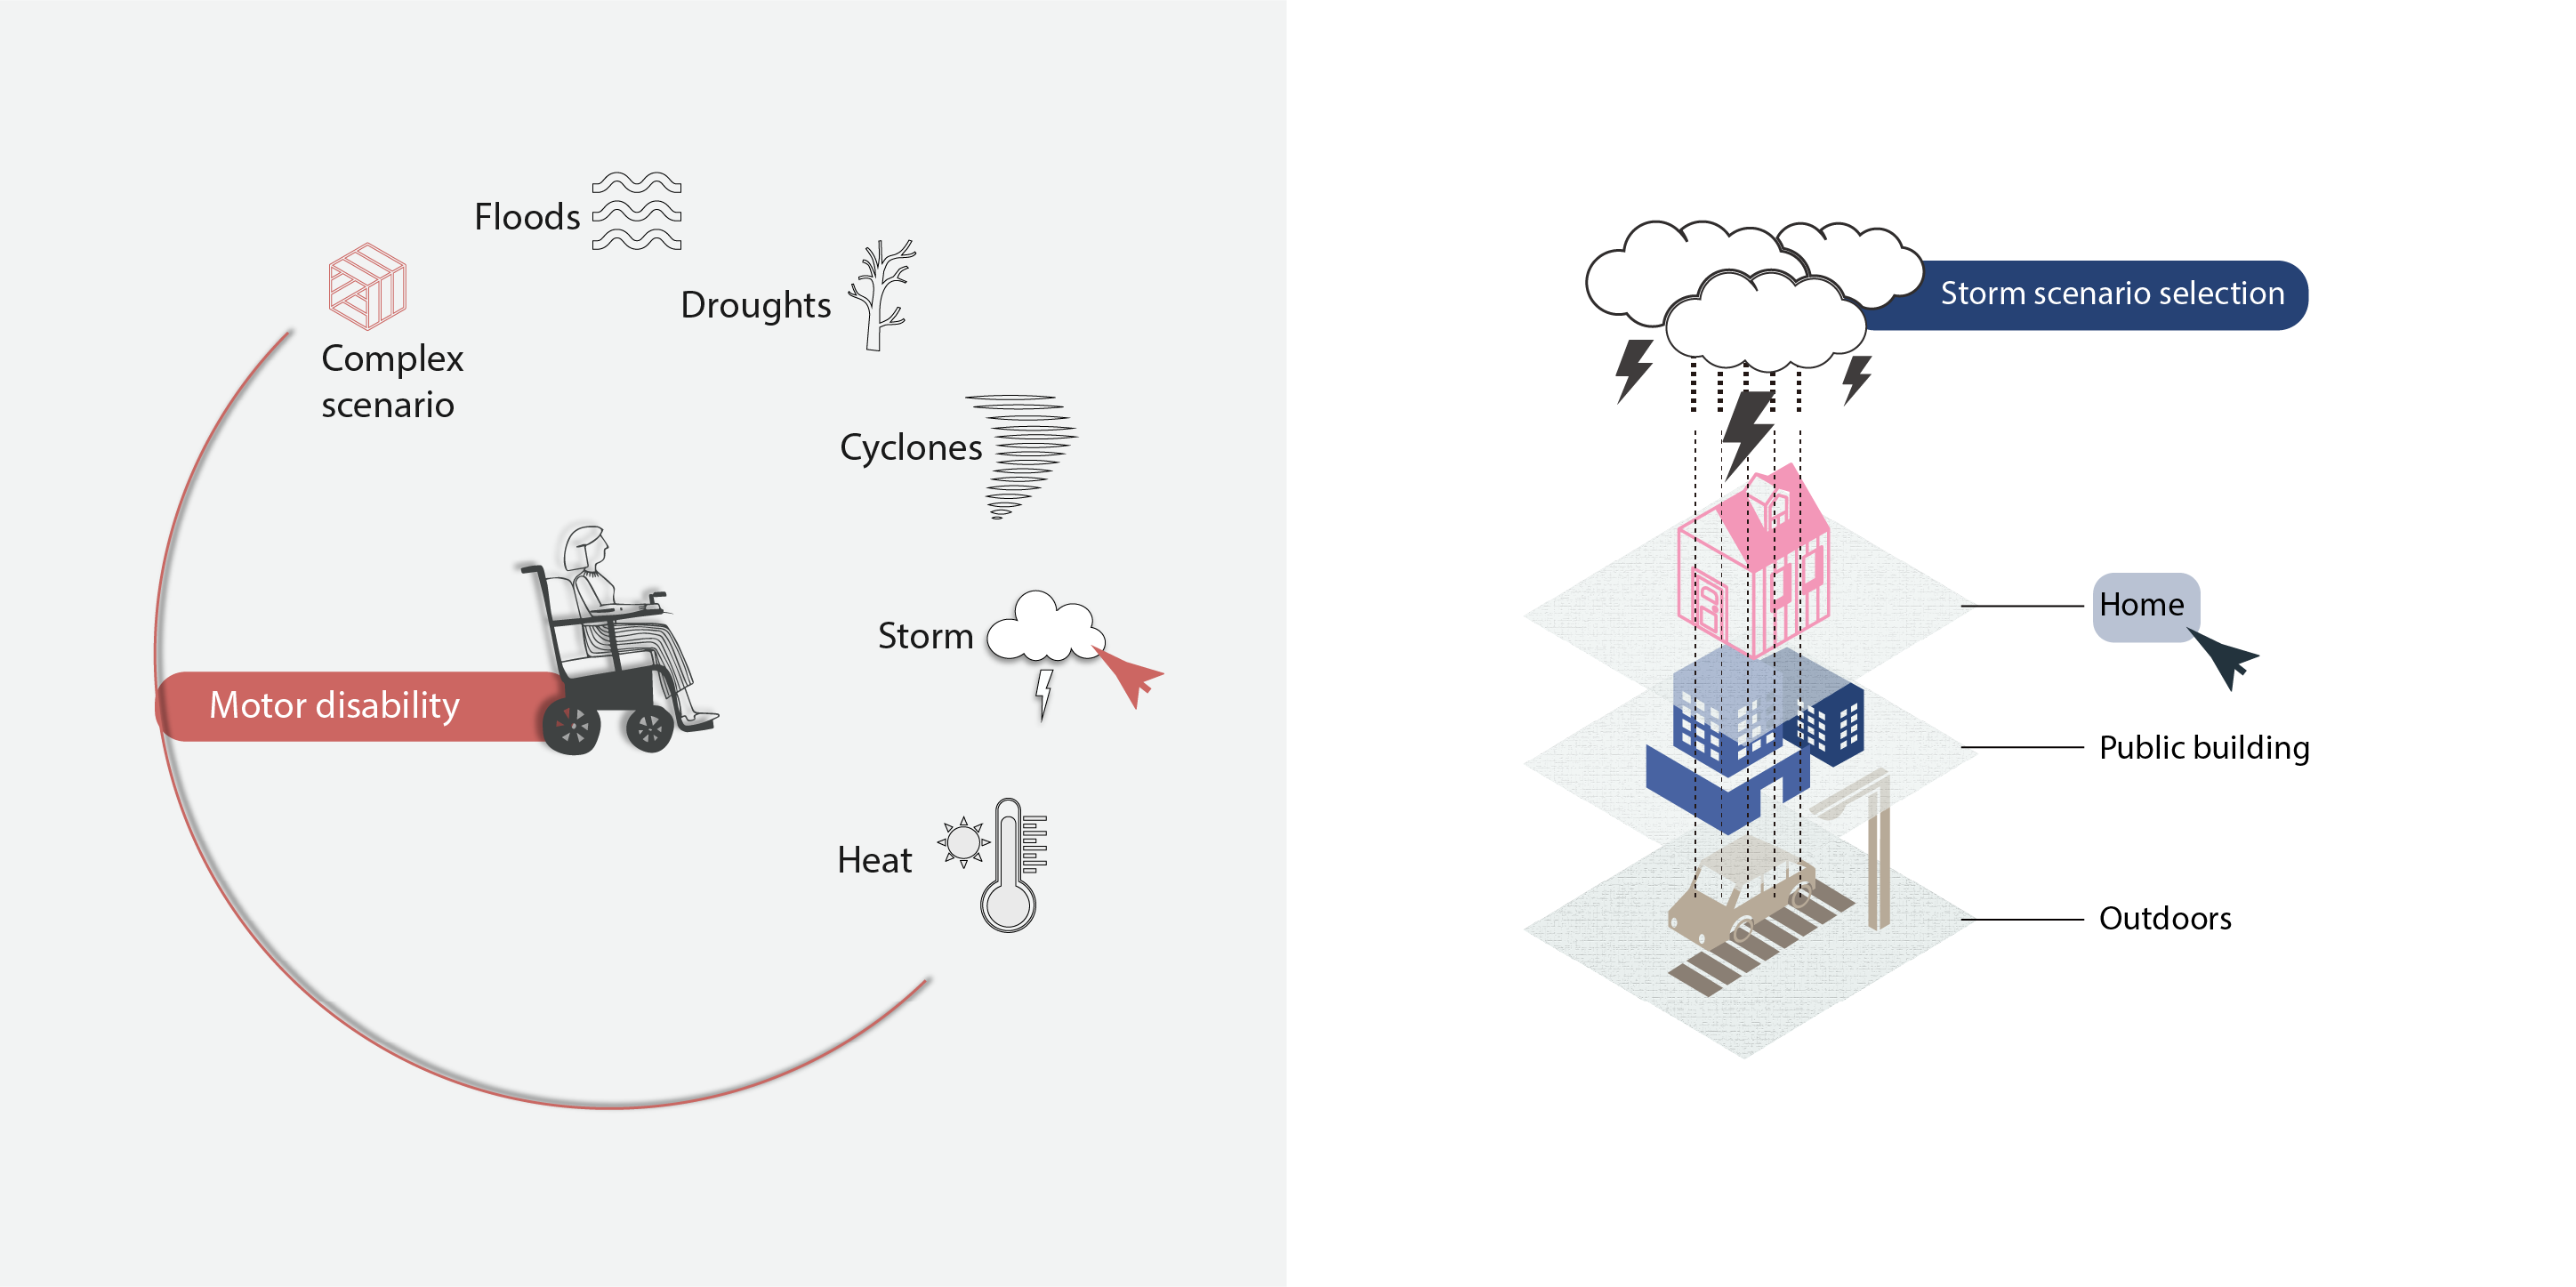
\includegraphics[width=\columnwidth]{Scenairo.png}
\caption{A frame from the urban-heatwave scenario, showing a decision
point in the narrative game.}
\label{fig:scenario}
\end{figure}

\section{Accessibility Design}
Accessibility is treated as a design requirement, not a post-hoc
adjustment, and is specified concretely for the first pilot round with
mobility-disabled participants. WCAG~2.2 Level AA provides the
accessibility target for the prototype, although formal conformance
testing remains future work. The prototype is designed to provide:
\begin{itemize}
\item \textbf{Input and motor.} Full keyboard operability for every
interaction; switch-access compatibility; large interactive targets
($\geq$44$\times$44\,px) with generous spacing; a non-pointer equivalent
for every pointer action. No interaction requires fine motor control,
drag, or multi-touch.
\item \textbf{Timing.} No time-limited decisions---heatwave urgency is
conveyed through narrative, not a countdown---so fatigue and variable
response times are accommodated. Sessions can be paused, saved, and
resumed.
\item \textbf{Perception and comprehension.} Screen-reader-compatible
markup and reading order; text alternatives for images; captions for
audio; minimum 4.5:1 text contrast; plain-language phrasing with optional
expansion of complex terms; no information conveyed by colour alone.
\item \textbf{Session and ethics.} Accessible consent; the right to
pause, skip, or withdraw at any point; scenarios screened to avoid
gratuitously distressing content. A remote option runs in parallel, not
as a fallback; in-person venues meet step-free access, accessible toilet
provision, and accessible transport routing.
\end{itemize}
Several requirements (screen-reader support, plain language, alt text)
exceed the strict needs of mobility-disabled players and are retained as
cross-cutting baselines that benefit participants with secondary or
co-occurring access needs. Accessibility and recruitment decisions are
made with DPO partners, so the research medium itself does not reproduce
the institutional normalisation the review identifies.

\section{Prototype}
The current prototype is an interactive Figma mock-up of the
urban-heatwave scenario, not a deployed software build, and is still in
development. It comprises X linked frames covering X of the seven
decision points described in Section~\ref{sec:game}, navigable through
clickable hotspots that branch between accessible and inaccessible
adaptation pathways. At this stage the prototype establishes the visual
language, narrative flow, and decision structure of the game; it is used
to elicit early feedback from disabled participants and DPO partners
before engineering effort is committed.

Its purpose is formative: to test whether the heatwave scenario reads as
realistic and relevant, whether the decision points are understandable,
and whether the interaction model is navigable. The prototype does
\emph{not} yet implement programmatic accessibility (screen-reader
semantics, keyboard/switch operability, save/resume); these are specified
in Section~4 as requirements for the engineered build and are not claimed
of the Figma artefact. Data capture, branching logic, and the analysis
pipeline are likewise future work.

\section{Formative Feedback from Two Disabled Participants}
%% SCAFFOLD --- replace [...] with real content; nothing here is asserted yet.
\textbf{Participants and method.} We gathered formative feedback from two
disabled participants [access needs], recruited through [DPO partner /
network]. Each took part in a [remote / in-person], [$\sim$X-minute]
session in which they [walked through the Figma prototype] and [thought
aloud / answered a short set of structured questions]. [Informed consent
was obtained; ethics status: \ldots] This is formative and qualitative;
we make no claims of generalisability from two participants.

\textbf{What we asked.} Sessions focused on three questions: (i) does the
urban-heatwave scenario read as realistic and relevant to their lived
experience? (ii) are the decision points understandable and the
interaction navigable? (iii) where does the design still exclude or
misrepresent them?

\textbf{What we heard.} % 3--5 short findings; one or two sentences each
\begin{itemize}
\item \emph{Relevance / realism:} [\ldots]
\item \emph{Understandability / navigation:} [\ldots]
\item \emph{Accessibility issues raised:} [\ldots]
\item \emph{Framing / representation:} [\ldots]
\item \emph{Requested changes / additions:} [\ldots]
\end{itemize}

\textbf{What we changed.} [1--2 sentences on concrete design changes
prompted by the feedback, or ``planned'' if not yet made.]

\section{Discussion}
This work reframes a problem usually treated as one of policy recognition
as a problem of accessible, participatory design. By translating four
empirically grounded mechanisms of exclusion into concrete design
requirements (Table~\ref{tab:bridge}), it offers a route from scattered
qualitative evidence on disabled people's adaptive decisions toward an
artefact that elicits such evidence directly and in a comparable form.
The narrative game positions disabled participants as decision-makers
rather than as subjects of risk assessment, and embeds DPO-led
participation as a structural feature rather than an accommodation,
addressing two mechanisms the review identifies as central.

Three limitations bound the contribution and are stated plainly. The work
is early-stage: the prototype is a Figma mock-up, and formative feedback
comes from two participants, so we make no claims of generalisability.
In-game choices are not identical to real-world behaviour; we treat the
game as a structured elicitation method, not a predictor of conduct under
actual climate stress. And the pilot deliberately scopes to one hazard
(urban heatwave) and one access group (mobility); extending to sensory,
cognitive, and communication-related needs is a design challenge in its
own right, since a single accessibility solution will not serve a
heterogeneous population. These constraints define the agenda rather than
undermining the approach.

\section{Conclusion and Future Work}
We have presented the design rationale for an accessible narrative game
that turns evidence of how disabled people are excluded from climate
adaptation into a method for generating decision-level behavioural
evidence with them. A mixed-methods review yielded four behavioural
mechanisms of exclusion; these were translated into concrete game-design
requirements and an accessibility specification, realised so far as an
interactive Figma prototype of a single urban-heatwave scenario and
shaped by formative feedback from disabled participants and DPO partners.

Future work proceeds along three lines. First, \emph{engineering}:
building the prototype into a deployable game that meets the WCAG~2.2 AA
target and undergoes formal conformance testing, with data capture and
branching logic implemented. Second, \emph{a DPO-co-designed pilot} with
mobility-disabled participants, followed by staged extension to sensory,
cognitive, and communication-related access needs against explicit
criteria. Third, \emph{analysis}: the behavioural and narrative data the
game generates will be analysed through Grounded Theory and topic
modelling, and the resulting concepts will inform an agent-based model
that evaluates the equity and effectiveness of disability-inclusive
adaptation policies. Together these steps move disability inclusion from
recognition toward testable, implementation-level design and evaluation.

\bibliographystyle{ACM-Reference-Format}
\bibliography{Reference}

\end{document}
